\section{Разработка программного продукта}

На этапе подготвки к разработке программного продукта, необходимо выбрать соответсвующие целям средства для разработки, а также составить
график разработки, ориентируясь на него в процессе работы.

\subsection{Инструментальные и программные средства разработки}

Чтобы приступить к разработке необходимо выбрать такие средства как:

\begin{enumerate}
    \item язык программирования;
    \item система контроля версий;
    \item хостинг кода;
    \item библиотеку для серверной части;
    \item библиотеку для написания GraphQL-сервера;
    \item систему упаковки приложения;
    \item редактор кода.
\end{enumerate}

\subsubsection{Язык программирования}

После проектирования было необходимо выбрать нужные Инструментальные и программные средства разработки.

Так как темой дипломного проекта являлась написание серверной части, то выбор состоял из трёх языков программирования: PHP, JavaScript(Node.js) и Python.

Ниже привидено краткое сравнение языков программирования и затем будут сделаны соответсвующие выводы:

\paragraph{Необходимые библиотеки и фреймоворки}

PHP: Обладает многими
фреймворками, такими
Symfony, Laravel и так
далее.

Node.js: Создан в первую
очередь для 
написания
серверных 
приложений. Однако сущесвуют такие фреймоврки как Express и Nest.js, которые облегчают разработку.

Python: Python имеет в
своём распоряжении
множество библиотек,
которые работают как
синхронно, так 
и асинхронно. Например, Django и aiohttp.

\paragraph{Стиль кода}

PHP: На момент сравнения
не было найдено
единого стандарта кода.

Node.js: Не обладает таким
стандартом.

Python: имеет PEP-8.

\paragraph{Документирование}

PHP: Имеет phpDocumentator,
но не входит в стандарт.

Node.js: Не обладает 
средством
автоматического 
документирования.

Python: Имеет в распоряжении 
pydoc, входящий в 
стандарт, 
единый принцип 
Docstringsи обладает
множеством линтеров.

\paragraph{Стиль исполнения}

PHP: Создаёт объект
приложения на каждый
запрос.

Node.js: Запускает единый 
сервер, где 
разрешает 
каждый запрос
соответсвующей
функцией.

Python: Схож с Node.js при использовании бекенд-фреймворк.

\paragraph{Выводы}

Исходя из вышесказанного был выбран язык программирования Python. Так как он относительно легок синтаксически, схож с Node.js по стилю исполнения,
имеет средство автоматической документации и входящий в стандарт PEP-8, что повывашает единообразие кода и выбор линтеров.

\subsubsection{Система контроля версий}

Системой контроля версий был выбран git, так как он является де-факто стандартом индустрии, несмотря на некоторые технические преимущества Mercurial.
По этой же причине с ним знакомы большинство разработчиков, поддерживающих открытое программноое обеспечение, что сэкономит время и финансы, если в проект
придут новые люди.

\subsubsection{Средство хостинга кода}

Необходимо было выбрать средсто хранения кода, так как это позволило бы работать с разных устройств, обмениваться наработками и коммитами и так далее.
Так как средством контроля версий был выбран git, то выбор стоял между GitHub, GitLab и Bitbucket.

Сравнение будет идти только между сообществом и встроенными возможностью CI и CD. Такой пункт как интерфейс является субъективным и не учитывается
в процессе выбора средств.

\paragraph{Сообщество}

GitHub: обладает большим сообществом разработчиков, вкладывающих в открыте проекта. Большинство библиотек расположены в GitHub.

GitLab: сообщество меньше, а GitLab больше используется в корпоративных целях чему способствует возможность распложить его на собственном сервере, иными словами
self-hosted.

Bitbucket: сообщество не развито, несмотря на что был одним из первых хостингов кода, работая изначально с Mercurial.

\paragraph{Возможности CI и CD}

GitHub: имеет простой и понятный, и бесплатный GitHub Actions. Семантически описывается в yaml файле; по синтаксису схож с docker-compose

GitLab: также имеет встроенный CI и CD, но в отлчии от GitHub Actions синтаксис простым назвать довольно трудно.

Bitbucket: тоже имеет CI/CD, однако бесплатные минуты значительно меньше, чем у GitHub.

\paragraph{Выводы}

Исходя из сравнения, выбор остановился на GitHub, так как он известен в сообщетсве открытого программного обеспечения, каковым является и configCastle и обладает встроенным
GitHub Actions, позволяющий автоматизировать рутинные задачи по запуску тестов после коммита.

\subsubsection{Библиотека для написания серверной части}

Исходя из требования к асинхронности программного продукта такие библиотеки как Django и Flask не рассматривались. Они работают в синхронном режиме, блокируя операции
ввода-вывода, а следовательно не подходят.

Одним из немногих кандидатов остался aiohttp, являющимся микро-фреймворком и работающем на встроенной библиотеке asyncio.

У aiohttp есть такие конкрунты как Sanic и FastAPI, однако количество дополнительных библиотек у них ограничено и сообщество не развито в достаточной мере.

\subsubsection{Библиотека для написания GraphQL-сервера}

Для того, чтобы реализовать GraphQL-сервер на Python можно воспользоваться двумя библиотеками:

\begin{itemize}
    \item Graphene;
    \item Tartiflette.
\end{itemize}

Был выбран Tartiflette, так как он:

\begin{itemize}
    \item асинхронный;
    \item работает с aiohttp;
    \item понимает язык sdl(schema definition language), являющимся родным для GraphQL.
\end{itemize}

\subsubsection{Система упаковки приложения}

Для того, чтобы доставлять код, библиотеки и прочие зависимости в удобном виде каждому человеку, не нарушая уже сложившуюся экосистему, сущесвует
два способа:

\begin{itemize}
    \item Виртуальные машины;
    \item Docker;
\end{itemize}

Виртуальные машины эмулируют работу железа и потребляют много ресурсов устройства, однако способны полностью воспроизводить ОС. Такое излишество неудобно, поэтому был выбран
Docker.

Docker ~--- это система виртуализации на основе хостовой операционной системы. Работает с такими терминами как образ и контейнер. В контейнер можно упаковать код и его зависимости, а затем
доставить этот контейнер в виде образа любому другому человеку или хостингу.

\subsection{Редактор кода}

В основном, используются специализированные редакторы кода, такие как vim, emacs, visual studio code, atom, sublime text и так далее.

В процессе разработки были выбраны такие редакторы как vim для быстрого написания непродолжительных участков кода, так как:

\begin{itemize}
    \item быстр;
    \item очень прост;
    \item позволяет очень быстро исправлять ошибки за счет своего управления.
\end{itemize}

Visual Studio Code был выбран потому что:

\begin{itemize}
    \item обладает большим колчеством расширений, так в работе использовалось расширение Docker, позволяющее управлять всей экосистемой прямо в редакторе;
    \item удобная система конфигурации настроек проекта, например, подключение линтера, в виде файла settings.json, который нужно расположить в отдельном каталоге.
\end{itemize}

\subsection{Календарный план разработки продукта}

В процессе проектирования был составлен предполагаемый график разработки проекта, представленный в таблице \ref{dev:date}.

\begin{longtable}[c]{|l|l|l|}
    \caption{План разработки продукта}
    \label{dev:date}\\
    \hline
    Этап работы                                      & Начало   & Окончание \\ \hline
    \endfirsthead
    %
    \multicolumn{3}{c}%
    {{\bfseries Table \thetable\ continued from previous page}} \\
    \endhead
    %
    Разработка требований                            & 01.11.19 & 15.11.19  \\ \hline
    Создание прототипов пользовательского интерфейса & 18.11.19 & 22.11.19  \\ \hline
    Написание прототипа сервера                      & 21.11.19 & 28.11.19  \\ \hline
    Создание дизайна                                 & 24.11.19 & 30.11.19  \\ \hline
    Разработка общей архитектуры проекта             & 01.12.19 & 13.12.19  \\ \hline
    Выбор технологий                                 & 15.12.19 & 20.12.19  \\ \hline
    Изучение документации к выбранным технологиям    & 21.12.19 & 25.12.19  \\ \hline
    Написание кода клиентской части                  & 24.12.19 & 17.04.20  \\ \hline
    Написание кода серверной части                   & 19.01.20 & 16.04.20  \\ \hline
    Тестирование клиентской части                    & 18.04.20 & 24.04.20  \\ \hline
    Тестирование серверной части                     & 22.04.20 & 25.04.20  \\ \hline
    Развёртывание на сервере                         & 26.04.20 & 29.04.20  \\ \hline
\end{longtable}

После составления графика была создана диаграмма Ганта, исходя из данных представленных в таблице \ref{dev:date}. Эта диаграмма показана на рисунке \ref{dev:gant_image}.

\begin{figure}[H]
    \center{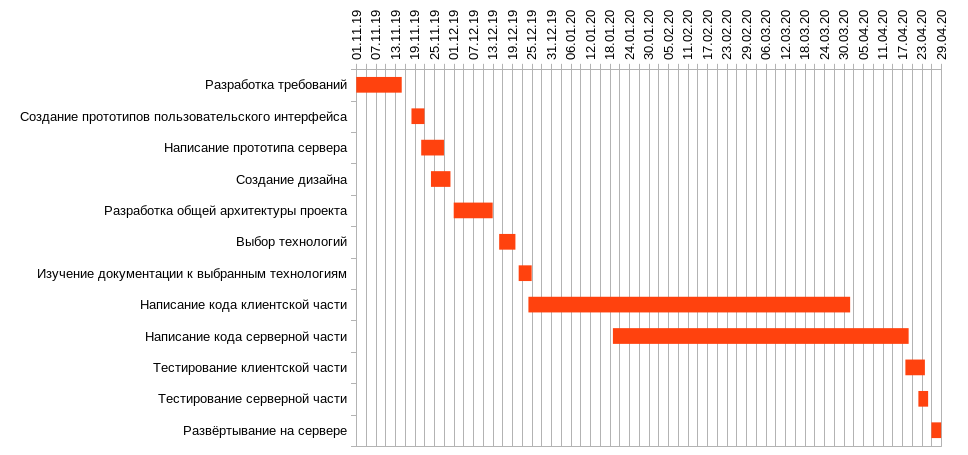
\includegraphics[scale=0.5]{gant.png}}
    \caption{Диаграмма Ганта}
    \label{dev:gant_image}
\end{figure}
